% Solution: Munoz-Garcia & Toro-Gonzalez (2019) Ch. 4, Exercise 9 "Centipede Game". Input by \solitem.
% New in the Lecture 3 practice list. Check: check_L03.py.
\begin{exsol}{\MG{} Ch.~4, Exercise 9}{176--177}{Foundations}{2}
\asked In the 100-stage centipede of Fig.~4.31: (a) the last mover's best reply; (b) the best reply
of the previous-to-last mover given (a); (c) the subgame-perfect equilibrium.

\method Backward induction on a long chain (Lecture~3, slides~59--64; Tadelis \S8.3.1 on the
centipede, pp.~159--160): the last mover's choice is the same at every history, so the argument for
stage $t$ is the argument for stage $t+1$ shifted by one. The text of the exercise says depositor~1 moves
at the 100th stage, but Fig.~4.31 and the book's answer have depositor~2 as the last mover, choosing between
$(99,101)$ and $(100,100)$; this solution follows the figure.

\solution
\textbf{The payoffs.} Read off Fig.~4.31, with $t = 1, \dots, 100$ the stage. Depositor~1 moves at odd stages,
depositor~2 at even stages. If the mover at stage $t$ stops (\emph{Stop}), the payoffs $(u_1,u_2)$ are
\[
  t = 2k-1\ (\text{depositor 1}):\ (2k,\ 2k-2), \qquad t = 2k\ (\text{depositor 2}):\ (2k-1,\ 2k+1),
\]
for $k = 1, \dots, 50$: $(2,0)$, $(1,3)$, $(4,2)$, \dots, $(97,99)$ at $t = 98$, $(100,98)$ at $t = 99$,
$(99,101)$ at $t = 100$. If depositor~2 continues at stage 100, the game ends at $(100,100)$.
\begin{center}
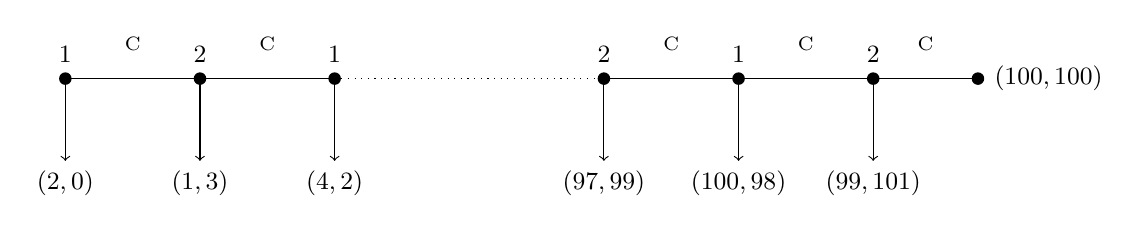
\begin{tikzpicture}[scale=0.95,dot/.style={circle,fill,inner sep=1.6pt},every node/.style={font=\small}]
  \foreach \i/\who in {0/1,1.8/2,3.6/1,7.2/2,9/1,10.8/2} {
    \node[dot,label=above:{\who}] (n\i) at (\i,0) {};
  }
  \draw (0,0) -- (1.8,0) -- (3.6,0); \draw[dotted] (3.6,0) -- (7.2,0); \draw (7.2,0) -- (9,0) -- (10.8,0) -- (12.2,0);
  \node[dot,label=right:{$(100,100)$}] at (12.2,0) {};
  \foreach \i/\p in {0/{(2,0)},1.8/{(1,3)},3.6/{(4,2)},7.2/{(97,99)},9/{(100,98)},10.8/{(99,101)}} {
    \draw[->] (\i,0) -- (\i,-1.1);
    \node[below] at (\i,-1.1) {$\p$};
  }
  \node[above] at (0.9,0.25) {\scriptsize C}; \node[above] at (2.7,0.25) {\scriptsize C};
  \node[above] at (8.1,0.25) {\scriptsize C}; \node[above] at (9.9,0.25) {\scriptsize C};
  \node[above] at (11.5,0.25) {\scriptsize C};
\end{tikzpicture}\\[2pt]
{\footnotesize Fig.~4.31 redrawn; down arrows are \emph{Stop}, horizontal arcs are \emph{Continue}
(stages 1--3 and 98--100 shown).}
\end{center}

\textbf{(a) The last mover (stage 100, depositor 2).} The subgame is a single choice:
\[
  u_2(\text{Stop}) = 101 > 100 = u_2(\text{Continue}) \;\Rightarrow\; \text{Stop}.
\]
This is the best reply whatever happened before: the last node is a proper subgame, so the history does not
enter the comparison.

\textbf{(b) Stage 99 (depositor 1).} Anticipating Stop at stage 100,
\[
  u_1(\text{Stop}) = 100 > 99 = u_1(\text{Continue}) \;\Rightarrow\; \text{Stop},
\]
because continuing leads to $(99,101)$, in which depositor~1 gets $99$.

\textbf{(c) Induction to the root.} Suppose that every mover from stage $t+1$ on stops. At stage $t$:
\begin{itemize}
  \item if depositor~1 moves ($t = 2k-1$), stopping pays $2k$, and continuing pays what he receives when
  depositor~2 stops at stage $2k$, namely $2k-1$: $2k > 2k-1$;
  \item if depositor~2 moves ($t = 2k$), stopping pays $2k+1$, and continuing pays what he receives when
  depositor~1 stops at stage $2k+1$, namely $2k$ (the payoff $(2k+2, 2k)$): $2k+1 > 2k$ (for $t = 100$,
  $k = 50$, continuing pays $100 = 2k$ in the same way).
\end{itemize}
The comparison always favors Stop by exactly one dollar, so Stop is optimal at every stage, down to the first:
$u_1(\text{Stop}) = 2 > 1 = u_1(\text{Continue})$ (continuing would let depositor~2 stop at $(1,3)$).
The unique SPE is the strategy profile in which \emph{each depositor plays Stop at every one of his
nodes}, on and off the equilibrium path; the outcome is $(2,0)$ at stage 1. It is the same for any length
of centipede. Uniqueness holds because every comparison is strict.

\interp Each player would gain from the other's cooperation: $(100,100)$ gives depositor~1 fifty times his
equilibrium payoff and depositor~2 infinitely more. But each stop is a best reply only because the other is expected to stop one step later,
and the chain of expectations starts from a last stage where cooperation has no future. Nash equilibrium
alone would not generate the paradox with such sharpness; backward induction does. The unraveling is
the same logic as the finitely repeated prisoner's dilemma (Lecture~5 and Tadelis Ch.~8--10).

\verify \texttt{check\_L03.py} builds the 100-stage tree with the payoff pattern above (checking the
printed payoffs $(2,0)$, $(1,3)$, $(4,2)$, $(97,99)$, $(100,98)$, $(99,101)$, $(100,100)$), runs backward
induction with exact integers, and asserts that every mover stops at every node, that each stop beats
continuing by exactly one dollar, and that the outcome is $(2,0)$; it repeats the check for lengths
$2, 4, \dots, 20$. Output line: \texttt{munoz-garcia-4-9: SPE = Stop at every stage; outcome (2,0); margin 1
everywhere}. \emph{Comparison with \MG{}'s answer} (pp.~177): it agrees, ending with
$\mathrm{SPNE} = (\text{Stop}_t, \text{Stop}_t)$ in every period $t$.

\mistakes
\begin{itemize}
  \item Following the text rather than the figure on who moves last: the figure has no payoffs for a
  depositor~1 move at stage 100.
  \item Describing the SPE by its outcome (``depositor 1 stops at once''): the strategy also says that
  every later mover would stop if reached.
  \item Arguing that a patient depositor 2 ``should wait'': at stage 2 he compares $3$ now with $2$ later,
  not with $100$.
\end{itemize}

\answer{(a) At stage 100 depositor~2 stops ($101 > 100$). (b) At stage 99 depositor~1 stops ($100 > 99$).
(c) The unique SPE has every depositor stopping at every node; the outcome is depositor~1 stopping at
stage 1, payoffs $(2,0)$.}
\end{exsol}
